\documentclass[10pt, a5paper, twoside]{jsarticle}

\usepackage{okumacro}
\usepackage{enumitem}
\usepackage{amssymb}
\usepackage{amsmath}{}
\usepackage{amsfonts}
\usepackage{amsthm}
\usepackage{bm}
\usepackage{url}
\usepackage{here}
\usepackage[dvipdfmx]{graphicx}
\usepackage{wrapfig}
\usepackage{makeidx}
\usepackage{braket}
\usepackage{ascmac}
\usepackage{fancyhdr}
\usepackage{tikz}
\usepackage[top=20truemm,bottom=20truemm,left=15truemm,right=15truemm]{geometry}

\pagestyle{fancy}
	\fancyhead{}
	\fancyhead[RE]{円城塔研究}
	\fancyhead[LO]{資料:コンメンタール「パリンプセストあるいは重ね書きされた八つの物語」}
	\fancyhead[LE, RO]{\thepage}
	\fancyfoot{}
	\fancyfoot[LE, RO]{\footnotesize{The Journal of EnJoeToh Research, Vol.2, No.1, 2024} }

\theoremstyle{definition}
	\newtheorem{axi}{公理}
	\newtheorem{dfn}{定義}
	\newtheorem{thm}{定理}
	\newtheorem{hyp}{予想}
	\newtheorem{ths}{提唱}


\begin{document}

	~ %強制改行

	\begin{center}

		\Large{コンメンタール「パリンプセスト\\あるいは重ね書きされた八つの物語」}

		\vspace{3mm}

		\large{Commentary of short story \textit{Palimpsest}}

		\vspace{3mm}
		
		\large{下村思游}

	\end{center}

	\vspace{3mm}

	\section{解説}

		頁数・行数は『ムーンシャイン』紙版\cite{moonshine}に準拠した.

		\subsection{題名}

			パリンプセストとは,使い古しの羊皮紙の表面を薄く削り,先に書かれていた文字を消して再利用したものに書かれた書物のこと.目視出来る範囲で削り取られていても,X線照射やインクの残存成分の科学分析から元の文書の内容を読み取れることがある.

			もちろん,“すべて”をそこに書き込んだという曽祖父の遺した文書に対する正しい言及であり,いかにかき消したとしても元の情報を復元可能であるという象徴としても機能する.

		\subsection{p.7, l.2-3}

			\begin{quote}

				「曽祖父は字送りというものを知らなかった人で,〜」
				
			\end{quote}

			冒頭から,いきなり面食らう文字列が提示される.作中の記述の通り,語り手の曽祖父は,字送りを知らなかったので,“すべて”を8個の正方形に書き込んだ.そこに”すべて”が書かれているのだが,そこに書かれた情報を取り出すことは出来ない.『Self-Reference ENGINE』で登場した,無限の文字列から情報を取り出すことは不可能である,という数学的事実と本質的に同一.

			一般に,物が破壊される,液体に別の液体が混ざり拡散する,という現象は不可逆である.しかしながら,拡散と破壊が行われるような系であっても,その系がどのように破壊されたかを調べることによって,どのように攪拌されたかを逆算することができる場合がある\cite{nkh}.

			この結果は,複雑で秩序構造を持たないはずの粘性流体から,秩序ある構造を取り出せることを意味しており,極めて興味深い現象である.なぜなら,秩序構造のない系から秩序構造のある系に遷移しており,一見エントロピーが減少しているように見えるからである\footnote{同様の事例として,複雑系としての癌細胞の振る舞いが挙げられる.単体の癌細胞はそれぞれ無秩序に増殖するが,なぜか総体として特徴的な秩序構造をとることがある.このような振る舞いに対しては,従来の病理学的なアプローチだけでなく,複雑系を扱うために培われた物理学的なアプローチが有効ではないかと期待されている.}.

			また,一箇所に“すべて”を書き込んだ,というモチーフからは江戸後期の越後の僧侶.良寛のエピソードが思い出される.良寛は書家としても有名であり,書の鍛錬を毎日欠かさなかった.あるとき,良寛の庵を訪ねた子供が,良寛が真っ黒な紙に向かって一心不乱に文字を書き続けていたところを見たという.良寛は,下手に文字を書くため,ボサボサの禿筆で同じ紙にずっと字を書きつけ,その紙が漆のように真っ黒に照り輝くようになっても鍛錬を続けていた\footnote{「余披而覧之,欣然曰,上人禅脱之余,尤好墨戯.余弱年嘗造其草庵,机上石硯禿筆,紙五六十張,皆黒如漆.」\\「余披いて之を覧,欣然として曰く,上人禅脱の余,尤も墨戯を好む.余弱年なりしとき嘗て草庵に造るに,机上石硯・禿筆・紙五六十張,皆黒きこと漆の如し.」\cite{ryo}}.

		\subsection{p.8, l.3}

			\begin{quote}

				「壁の中にいる.」
				
			\end{quote}

			コンピュータRPGの古典『Wizardry』の有名なメッセージ.

			Wizの宝箱の罠としてテレポーターというものがあり,これに引っかかってしまうと,マップ上のどこかにランダムに転送されてしまう.このメッセージは転送先に空間がない場合(=壁の中など)のもので,この場合パーティメンバーは即死・消滅し,ゲーム内から完全に失われてしまう.

		\subsection{p.8, 16-17}

			\begin{quote}

				「ただのDNAの連なりがただの化学物質でしかないように,〜」
				
			\end{quote}

			遺伝情報を記録するDNAであっても,それを読む者がなければ,ただの糖鎖にすぎない.円城塔が「考速」\footnote{ハヤカワ文庫JA『後藤さんのこと』収録.「あるいは,不意に目の前に投げ出された脳みそを,絡み合う矢印の山と見なして解きほぐすこと.だから順序は逆転される.定義と公理が与えられ,推論規則を用いて定理が導き出されるわけではなく,相互に作用する網目がまずあり,推論規則が見定められ,定理の形が決定されて,定義と公理が抽出される.」\cite{goto}p.113}「ガベージコレクション」\footnote{ハヤカワ文庫JA『後藤さんのこと』収録.今目の前にある事物がいかにしてここにあらしめられたのかや,可逆計算に関する議論など,様々なスケールにおける熱力学的に基づく逆問題,あるいは“記述すること”によって記述出来るものと失われるものについて考察する.「何かが理解可能であるかどうかは,科学の範疇には属さない.理解できるものを理解するのが,科学の役割であるからだ.この言が不適切だとされるなら,理解できたものしか語らないのが科学であるから.原理的に理解のできないものに対しては,せいぜい理解不可能であると理解するのが科学の上げることのできる得点だ.科学は理解不可能なものを理解可能な対象へと切り替える機能を持っておらず,これはあまりにも当然すぎる.」\cite{goto}p.147}「バナナ剝きには最適の日々」\footnote{ハヤカワ文庫JA『バナナ剝きには最適の日々』収録.}「内在天文学」\footnote{河出文庫『シャッフル航法』収録.}などの作品で明示する経験論\footnote{“対象”は“観測者”によって“観測”されることによって初めて科学の扱える対象になるのであり,そうでなければ存在するかどうかを問うこと自体が科学的に無意味である,という立場.現代の物理学者のほぼ全員がこの立場をとる.円城塔は経験論的立場をしばしば明確に表明しているのだが,作中の数理科学的に難解な記述に隠蔽され,見えづらくなっているように感じられる.この立場を明確にしていることにより,衒学的な作風でありつつも,いわゆるポストモダン的な濫用に陥っていないのだと考えられる.}的立場を,ここでも明示している.

			文字列を外部の観測者が読む,あるいはより抽象化して,何らかの配列と外部の系が相互作用することによって,その配列の上を走る“計算”が駆動し,“物語”が展開する,という構造が円城塔作品には頻出する.無論,本作「パリンプセスト」がその好例であり,同書収録の「ムーンシャイン」のほか,「十二面体関係」,「ドルトンの印象法則」\footnote{柏書房『夕暮れの草の冠』収録.『春と修羅』序文の各文字を入れ替えたものを,より乱雑なものから多少文意が通るものまで複数パターンを順番に提示し,文意が立ち現れる過程を示す.}などが挙げられる.また,相互作用というモチーフは,本作の後半でホイーラー--ファインマン吸収体理論に結実する.

		\subsection{p.10, l.4-5}

			\begin{quote}

				「一次元格子の上に無限に並べられた点の数と,平面格子に敷き詰められた点の数は,厳密な意味で一致する.」
				
			\end{quote}

			作中の“無限”が可算無限を指すのだとすれば,これは数学的に正しい.一次元格子上の点の集合の濃度$n$と平面格子上の交点
			の集合の濃度$n^2$は$n, n^2 \in \mathbb{N}$のとき一致する.

			$n$と$n^2$の“大きさ”が一致するというのは一見意味不明な主張だが,下図のような方法を用いるとわかりやすい.

			\vspace{2mm}

			\begin{center}
				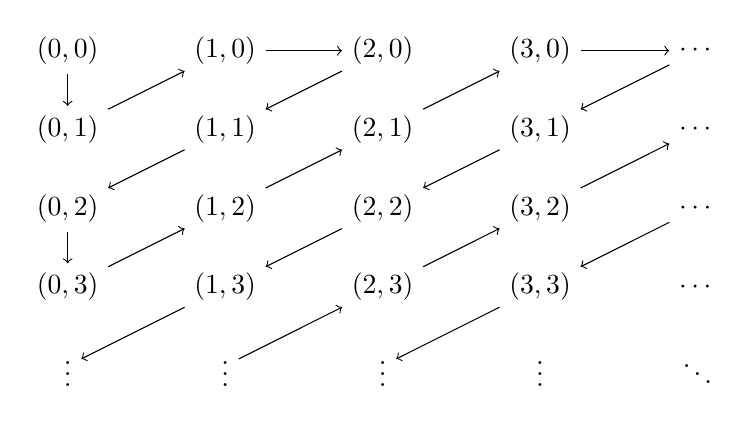
\begin{tikzpicture}[auto]\label{arrows}
					\node (pt00) at (0,  0) {$(0, 0)$};
					\node (pt01) at (0, -1) {$(0, 1)$};
					\node (pt02) at (0, -2) {$(0, 2)$};
					\node (pt03) at (0, -3) {$(0, 3)$};
					\node (dots04) at (0, -4) {\vdots};

					\node (pt10) at (2,  0) {$(1, 0)$};
					\node (pt11) at (2, -1) {$(1, 1)$};
					\node (pt12) at (2, -2) {$(1, 2)$};
					\node (pt13) at (2, -3) {$(1, 3)$};
					\node (dots14) at (2, -4) {\vdots};

					\node (pt20) at (4,  0) {$(2, 0)$};
					\node (pt21) at (4, -1) {$(2, 1)$};
					\node (pt22) at (4, -2) {$(2, 2)$};
					\node (pt23) at (4, -3) {$(2, 3)$};
					\node (dots24) at (4, -4) {\vdots};

					\node (pt30) at (6,  0) {$(3, 0)$};
					\node (pt31) at (6, -1) {$(3, 1)$};
					\node (pt32) at (6, -2) {$(3, 2)$};
					\node (pt33) at (6, -3) {$(3, 3)$};
					\node (dots34) at (6, -4) {\vdots};

					\node (dots40) at (8,  0) {$\cdots$};
					\node (dots41) at (8, -1) {$\cdots$};
					\node (dots42) at (8, -2) {$\cdots$};
					\node (dots43) at (8, -3) {$\cdots$};
					\node (dots44) at (8, -4) {$\ddots$};


					\draw[->] (pt00) to node {} (pt01);

					\draw[->] (pt01) to node {} (pt10);

					\draw[->] (pt10) to node {} (pt20);

					\draw[->] (pt20) to node {} (pt11);
					\draw[->] (pt11) to node {} (pt02);

					\draw[->] (pt02) to node {} (pt03);

					\draw[->] (pt03) to node {} (pt12);
					\draw[->] (pt12) to node {} (pt21);
					\draw[->] (pt21) to node {} (pt30);

					\draw[->] (pt30) to node {} (dots40);

					\draw[->] (dots40) to node {} (pt31);
					\draw[->] (pt31) to node {} (pt22);
					\draw[->] (pt22) to node {} (pt13);
					\draw[->] (pt13) to node {} (dots04);

					\draw[->] (dots14) to node {} (pt23);
					\draw[->] (pt23) to node {} (pt32);
					\draw[->] (pt32) to node {} (dots41);

					\draw[->] (dots42) to node {} (pt33);
					\draw[->] (pt33) to node {} (dots24);
				\end{tikzpicture}
			\end{center}

			このように,2次元平面上の格子点をジグザグに辿っていくことで,すべての格子点を1次元直線上の格子点と1対1に対応させることが出来る.つまり,$n$と$n^2$の間に全単射があるので,これらの濃度は一致する.

		\subsection{p.12, l.3-10}

			\begin{quote}
				「\texttt{empty = "A"}〜」
			\end{quote}

			プログラミング言語Rubyによるコード.本来Rubyは\texttt{while}を多用しなくてもいいような言語設計になっており,\texttt{while}を書くときは無限ループを書くときに限られる.実際,ここでは無限ループを書いており,Rubyらしさを崩してでも無限ループを明示的に書いたことが認められる.

			このコードは,\texttt{long}を無限個集積したのち,\texttt{time ago.}と繋げて出力させる.無論,無限個の\texttt{long}を積みきることはないので,シークエンスは終了せず無限ループする.コード自体はきちんと完結しているが,コードを解釈することによって得られる処理はループする.コードという配列と,その解釈によって駆動する“計算”という構造がここにも明白に見られる.

		\subsection{p.13, l.1-5}

			\begin{quote}

				「あなたがこの段落に〜」
				
			\end{quote}

			ここに辿り着けたのであれば,読者は本文で指摘されているいずれかの状態を満たしている.“すべて”の始めも始めに脱出不能の罠を仕掛ける曽祖父の狡猾さ,あるいは読み手側の猜疑心を反映するか.あるいは『Wizardry』であれば当然身構えておくべきこと\footnote{先述のテレポーターの罠は,ゲームの最序盤でも登場する.}.

		\subsection{p.13, l.6}

			\begin{quote}

				「ようこそ,一番最初の無限の果てのこちら側へ.」
				
			\end{quote}

			文字通り,我々は無限を超えてすぐの地点にいる.通常“無限”と呼ばれるものは,数学では可算無限と呼ばれるもので,その名の通り,無限ではあるが数え上げられる程度の無限でしかなく,“一番最初の無限”である.また可算無限より“大きい”無限が存在し,不可算無限という.

			“こちら側”として適当な,より大きな無限の例として巨大基数である弱到達不能基数・強到達不能基数が挙げられ,これらは以下のように定義される\cite{arai}.

			\begin{dfn}

				弱到達不能基数・強到達不能基数の定義

				弱到達不能基数$\kappa = \aleph_\alpha$とは,極限基数,つまり$\alpha$が極限順序数でしかも正則であるような基数のことである.

				強到達不能基数とは,非可算$\kappa > \aleph_0$で正則かつ強極限基数となっている基数$\kappa$のことである.
				
			\end{dfn}

			弱到達不能基数・強到達不能基数は,いずれも集合論の公理であるZFC公理系からは証明出来ない.また,弱到達不能基数・強到達不能基数は一般連続体仮説の下で一致することが知られている.

		\subsection{p. 14, l.9}

			\begin{quote}

				「そこには全てがあるせいで,多重の砂絵の中から好きな映像が取り出されうる.」
				
			\end{quote}

			ウィリアム・ギブスン『ニューロマンサー』の冒頭\footnote{「港の空の色は,空きチャンネルに合わせたTVの色だった.」\cite{neuro}p.11}を思い出す.なお,この主張自体は前述の通り詭弁である.

		\subsection{p.16, l.11-15}

			\begin{quote}

				「宝玉の来訪と非来訪は〜」
				
			\end{quote}

			宝玉を用いたアナログなデジタル通信に違いない,という確信を得られる記述.

		\subsection{p.18, l.16-17}

			\begin{quote}

				「都が砂の波に〜」
				
			\end{quote}

			回路に想定よりも多くの電子が流入してしまうことは,電子回路が故障したり誤作動することの原因である.一般的には,放射線が原因であることが多い.

		\subsection{p.20, l.4-6}

			\begin{quote}

				「それぞれの穴から〜」
				
			\end{quote}

			迂遠なプログラミングであり,中国脳\footnote{哲学における思考実験.無数の中国人を用意し,通信機器と,入力に対して出力するべき信号のリストを渡す.この中国人たちが脳の神経細胞のネットワークを忠実に再現するならば,この中国人たちから成る脳に意識はあるだろうか,というもの.}でもある.

		\subsection{p.22, l.1-3}

			\begin{quote}

				「涙が方程式に従わないという見解は,〜」

			\end{quote}

			還元主義.生物学は化学で,化学は物理学で記述されるというのは妥当な推論だが,どこまで徹底するかは議論の余地がある.本作では,還元主義をさらに推し進め,物理学を数学に還元し.数学に規律される生理現象を扱う.これは,後述する認知論に関するデュ・ボア・レーモンの立場とヒルベルトの立場を折衷したものとなっている.

		\subsection{p.23, l.6-8}

			\begin{quote}
				
				「機械支援をうけた定理証明自体はさして珍しいことではないが,〜」
				
			\end{quote}

			代表的な定理証明支援系言語としてCoq\footnote{フランス国立情報学自動制御研究所を中心に開発・管理されている定理証明支援系.プログラミング言語OCamlで書かれたソフトウェアであり,電子計算機上で動作する.}が知られており,これを用いた数学の証明として有名なものに四色定理とファイト--トンプソンの定理(奇数位数定理)がある.

			また,機械支援を受けた数学はさして珍しいことではない,というのは(分野にもよるが)事実である.

		\subsection{p.23, l.15}

			\begin{quote}
				
				「要するに笑いすぎて死んだ.」

			\end{quote}

			モンティ・パイソンの有名なスケッチ「殺人ジョーク」が元ネタ.

		\subsection{p.25, l.5-6}

			\begin{quote}
				
				「ところで,活字を見て涙を流す,それではなにかあんまりなので,文章を見て涙を流すという過程には,何か奇妙なものが存在する.」

			\end{quote}

			これが不思議なことに異論はない.人間の認知機構は古くから探究されているが,様々な困難によって未解決となっている問題が多く存在する,ここでは,円城塔作品の読解に有用であると考えられる,エミール・デュ・ボア・レーモンによる不可知論とそれへの反応について紹介したい.

			デュ・ボア・レーモンは,ヘルムホルツ\footnote{熱力学におけるヘルムホルツの自由エネルギーなど,物理学者としての功績で非常に有名だが,生理学者・哲学者としても多大な功績がある.最後の自然哲学者とも言える.}とともに19世紀における生物学・生理学の物理学化に大きな貢献をした生理学者である.デュ・ボア・レーモンは,精神の根源と考えられる人間の神経の物理的な構造を研究する一方で,人間の認知機構を含め,自然科学には原理的に探れないような領域があると主張した\footnote{Ignoramus et ignorabimus. 我々は知らない,我々は知ることはないだろう.円城塔作品に神経細胞を擬人化した「イグノラムス・イグノラビムス」という作品があるのは偶然ではない.}\cite{hys,dbr}.

			これに触れた若き日のヒルベルトは,真偽が決定不能な領域を抱えうる体系に敵意をあらわにし,数学においてはそのような問題が起こらないということを数学自身によって証明することで,数学の完全性と無矛盾性を確認するヒルベルトプログラムをやがて提唱することになる.しかし,ヒルベルトプログラムは,第一不完全性定理を証明したゲーデルによって,駆動した直後に破綻することになった.決定不能なことが存在するというデュ・ボア・レーモンの主張に反発し,決定不能なことなどないと証明しようとしたヒルベルトの試みが,決定不能なことは存在するというゲーデルの主張によって破れたことは,極めて興味深い.

			また,円城塔は,人間の認知機構を攻撃し,特定の情動を引き起こすような小説について何度か指摘している\cite{kbd,eql}ことにも注意したい.

		\subsection{p.25, l.8}

			\begin{quote}
				
				「灰色の脳細胞」

			\end{quote}

			アガサ・クリスティの創作した名探偵,エルキュール・ポアロの口癖に由来するか.“知的遊戯”としてのミステリから引くことで,人間の知的活動の根源である脳細胞を強調する意図があると考えられる.

		\subsection{p.25, l.10}

			\begin{quote}
				
				「エネルギー収支をどこで追えばよいのかよくわからない.」

			\end{quote}

			これは本当にそう.テクスト--読者から成る系と,その間の相互作用として読書をとらえようとする問題意識は,円城塔作品の中でも特に2020年代以降の作品に頻出する.ここにその萌芽が認められることは,円城塔の問題意識が初期から一貫していることを示す.

		\subsection{p.26, l.18-p.27, l.1}

			\begin{quote}
				
				「ほどなく彼らは,抽象関係を文字や映像に混入して流通させることに成功する.」

			\end{quote}

			サブリミナル効果.現代ではその効果は否定されている.

		\subsection{p.28, 5-7}

			\begin{quote}
				
				「人間の言語神経網を模した国語学研究所計算クラスタは涙多様体の発見をこそ導いたが,そこに知性の萌芽らしきものは未だ発見されていない.」

			\end{quote}

			ニューラルネットワーク.ここでの記述に反して,いまや現実には人と区別のつかない生成AIが溢れている.

			また,巨大で複雑なものが知性を持つという主張は,「ムーンシャイン」でも見られる.

		\subsection{p.29, l.3}

			\begin{quote}
				
				「そして青い液状の物質を,レンズへ向けて噴射してやった.」

			\end{quote}

			青いレンズは「Boy's Surface」\footnote{ハヤカワ文庫JA『Boy's Surface』収録.人間と人間の間の関係,特に恋愛関係を数理モデルとして扱う.}にも登場する(トルネド).また,トルネドは青い証明であるので宮沢賢治『春と修羅』(青い照明)も自動的に連想される.

		\subsection{p.30, l.1}

			\begin{quote}
				
				「「」

			\end{quote}

			「これはペンです」\footnote{新潮文庫『これはペンです』収録.「叔父は文字だ.文字通り.」から始まり,最終的に本作の語り手が本文テクスト全体であったことが示される.}のような,本文の内容が本文全体を引数に持つような仕掛けが施されている.また,「for Smullyan」で明記される対角化が既にここで用いられていることもわかる.無論,自己言及である.

		\subsection{p.32, l.6}

			\begin{quote}
				
				「は,今日も相変わらず「手を伸ば」し続けている」

			\end{quote}

			「これはペンです」のオチの同類.

		\subsection{p.32, l.7}

			\begin{quote}
				
				「何故分かるように話さないの.」

			\end{quote}

			『AUTOMATICA』\footnote{ハヤカワ文庫『バナナ剝きには最適の日々』収録.題名,著者名,テクスト本文を互いに交換して$3!$通りの読み方で読めることを主張し,体現するテクスト.ジェラール・ジュネットが『スイユ』で行った,テクスト--パラテクストの対比をひっくり返すことを意図したか.}で見られる,文章の主体--客体関係をひっくり返して見せる悪戯.これは,フレーゲ--ラッセルによる記述の理論から,命題の主客を転倒させても意味が保存される可能性があるという議論を引かれてきたもの.

		\subsection{p.39, l.8}

			\begin{quote}
				
				「かなりのところ我慢強い.」

			\end{quote}

			クマムシに由来するか.


		\subsection{p.41, l.5}

			\begin{quote}

				「量子力学という古典理論」
				
			\end{quote}

			普通,物理学において古典理論とは,ニュートン力学のことを言う.ニュートン力学(狭義の古典力学)と,それと等価な理論である解析力学を合わせて(広義の)古典力学といい,古典力学--量子力学という観測理論を軸とした対応関係がある.一方で,時空を記述する理論として古典力学--相対論という対応関係がある.古典力学では運動理論・観測理論・時空の記述が一体として体系化されていたが,運動理論・観測理論である量子力学と,時空の記述を司る相対論の融合は,特殊相対論と量子力学の融合である相対論的量子力学の構築までに留まっており,重力理論を司る一般相対論が取り残される形となっている.

			あるいは,量子力学自体が,日常的な感覚では古典と言えるほど古いという事実からか.初期量子論の萌芽は1900年に発表されたプランクの黒体輻射の研究にあり,数学的な整備がなされたのも1925年のハイゼンベルクの行列力学,シュレーディンガーの波動力学であり,優に100年の歴史を有する.

		\subsection{p.42, l.13-14}

			\begin{quote}
				
				「直感がそれを否定しようとも,その場合は直感側が間違っている〜」

			\end{quote}

			経験科学としての物理学の本質である.直前にもあるとおり,実験事実からその正しさが明らかになりつつあった相対論や量子論を受容するにあたって,物理学者は極めて大きな苦しみを味わうことになった.相対論や量子論の示す事実に基けば,何かが確かに“在り”,ずっと在り続けることはないのである\footnote{今ここに何かが実在するということを物理学的に厳密に定義したものを局所実在論という.EPRパラドックスとベル不等式から導かれる局所実在論の否定について,詳しくは\cite{ein}を参照されたい.量子力学の標準的な教科書としては,公理的な教科書として\cite{smz}を,総覧的教科書として\cite{igkw}を参照されたい.}.この衝撃について,科学哲学では“物理学の危機”といい\cite{noe},ゲーデルの第一不完全性定理を発端とする“数学の危機”とともに人間理性の限界を示すものであるとして(過大に)評価されたが,当の物理学は危機を軽く乗り越え発展を続けた.

		\subsection{p.43, l.5}

			\begin{quote}

				「ヤン=ミルズ多様体」
				
			\end{quote}

			ヤン--ミルズ理論,ヤン--ミルズゲージ理論ではない何か.ヤンとミルズの名前だけを借りた造語か.

		

		\subsection{p.43, l.9}

			\begin{quote}
				
				「人生方程式」

			\end{quote}

			内容は物理学的・数学的にまあまあ真っ当なことが書いてあるが,名前が胡散臭すぎる.この命名は,物理学会や数学会に時折出没する似非科学から引かれたものだろう.例えば,任意の問題に対して正解を出せるのだが,そのための入力は依然として知れないという傑作,万能方程式が挙げられる\cite{irmn}.


		\subsection{p.45, l.9}

			\begin{quote}

				「ホイーラー・ファインマン吸収体理論」
				
			\end{quote}

			こちらは実在する物理学の理論.物理学的な説明は文中にある通り.直後に「その帰結は,一体の観測者もいない場合に,星は輝くことできないことを示唆する」\footnote{これは後で引用するファインマン本人の言葉をいくつか貼り合わせたものであるが,その大元はファインマン以前に同様の理論の構築に励んでいた夭折の物理学者ヒューゴー・テトローデの論文である.「宇宙にただ一つだけ太陽が存在し,他の天体がその輻射を受け取れないならば,太陽は輝かない.」\cite{tet}}とあるが,これも同様に正しい.以下,ホイーラー--ファインマン吸収体理論(以下,WF理論)を概説する.

			WF理論は,量子力学に電磁相互作用を導入した拡張理論である,量子電磁気学における困難(もし電荷が自身の作る電磁場と相互作用するなら,点電荷の質量は無限大でなければならない)を回避するために構築された理論である.この困難を回避するためには,電荷の質量を考えてはならないか,あるいは荷電粒子は全て空間的に広がっていなければならない.前者は量子力学そのもので,後者は相対論で即座に否定されるため,どちらの解決法も認め難い.そこで,ファインマンは,そもそも電荷は自己相互作用しないのではないか,との考察を学部生時代に行い,指導教官のホイーラーとともに卒業論文にまとめた.

			ファインマンによれば,その帰結は以下の通りとなる\cite{thesis}.

			\begin{quote}

				「何もない空間に孤立した原子は,実は輻射を起こさない.輻射は他の原子(すなわち,輻射を吸収する物質の中のもの)との相互作用の帰結である.すると量子力学での原子の自発放出もまた自発的ではなくて,他の原子に誘発されたものであるかもしれない.さらに光の見かけ上の量子的な特性すべてと光子の存在は,物質同士が直接量子力学の法則に従って相互作用することの結果に過ぎないかもしれない.」
				
			\end{quote}

			これはいわゆる量子力学の観測者問題なる疑似問題に近い話題だが,そもそもWF理論には量子力学を要請していないことに注意したい.上記の帰結は,古典電磁気学を適当に解釈することで得られる.本理論の物理学的な詳細は,末尾の参考文献を適宜参照されたい.

			さて,WF理論について説明したのは,ファインマンによる帰結が円城塔作品の本質をついた言及となっているからである.つまり,ファインマンの帰結をこう読み換えたい:孤立したテクストは,実は物語を生み出し得ない.物語はテクストと読者との相互作用の帰結である.

			テクストという対象があり,それが読者と相互作用を起こすのであれば,そこに物理を見るのは当然である\footnote{無論,読まれないときのテクストと物語の振る舞いを考察するのも当然である.}.誰かに読まれてしまった結果,悲惨な結末を迎える「十二面体関係」\footnote{朝日文庫『20の短編小説』収録.},ひとりでに駆動し続けることになってしまった「Self-reference ENGINE」\footnote{ハヤカワ文庫JA『Self-Reference ENGINE』収録.},物語に書かれてしまったことで生と死を規定されてしまった登場人物について考察する「墓の死」\footnote{『新潮』2021年9月号掲載.ここで扱われる問題は後期クイーン的問題の一般化と言えるかもしれない.ただし,後期クイーン的問題は法月綸太郎によって(柄谷行人を経由した)誤解に基づいた第一不完全性定理的な何かが導入されて議論が不明瞭になっているのに対し,円城塔は常に厳密である.あるいは,ハイデガーから,読者によって物語の中に投げ込まれた人物に関する考察と言った方が正確かもしれない.}など,円城塔作品には読まれることについての作品群がある.

		\subsection{p.46, l.1-2}

			\begin{quote}

				「このところ数が数えられなくなってきていて,〜」
				
			\end{quote}

			グロタンディーク素数を連想する.20世紀最大の数学者,アレクサンドル・グロタンディークは,ある議論において素数の例として57を挙げ,何事もなかったかのようにそのまま議論を続けたという.もちろん$57 = 19 \times 3$は合成数であり素数ではないのだが,グロタンディークが素数というなら素数であり,57をグロタンディーク素数というようになった.

		\subsection{p.46, l.10-12}

			\begin{quote}
				
				「数を数えるとはその数一つでできることではなくて,(中略)数を数えるにはその一つ前の数を覚えていなければはじまらない.」

			\end{quote}

			ペアノの公理のこと.ペアノの公理とは,公理集合論における自然のモデルで,以下のように定義される.

			\begin{axi}

				ペアノの公理

				\begin{enumerate}
					\item 自然数$0$が存在する.

					\item 任意の自然数$a$に対して,その後者である$S(a)$が存在する.

					\item $0$はいかなる自然数の後者でもない.

					\item 異なる自然数は異なる後者をもつ.

					\item $0$がある性質をもち,$a$がある性質を満たせばその後者$S(a)$もその性質を満たすとき,すべての自然数はその性質を満たす.
				\end{enumerate}
				
			\end{axi}

			このようにして,自然数は,0を規定としてそこに1を足し上げていったものとして定義される.すなわち,数えられることが数の数たる根拠である.

		\subsection{p.48, l.7}

			\begin{quote}

				「少なくともコンパクトにできている.」
				
			\end{quote}

			人間の体を,人間の体を構成する要素を集めた集合で表すと,その集合は有限集合になる.つまり,コンパクトである.この“コンパクト”は数学の用語であり,以下のように定義される\cite{hara}.

			\begin{dfn}

				コンパクト

				位相空間$X$の部分集合$A$の任意の開被覆$\{ O_\lambda \}_{\lambda \in \Lambda}$が有限被覆を部分集合として持つとき,すなわち,開集合の族$\mathcal{O} = \{ O_\lambda \}_{\lambda \in \Lambda}$について$A \subset \bigcup_{\lambda \in \Lambda} O_\lambda$ならば,その有限個の開集合$O_1, \cdots O_n \in \mathcal{O}$$でA \subset O_1 \cup \cdots \cup O_n$となるものがあるとき,$A$はコンパクトであるという.
				
			\end{dfn}

		\subsection{p.50, l.1-5}

			\begin{quote}

				「あなたが本を見ていない間でも,本に書かれていることは変わらない.〜」

			\end{quote}

			テクスト--読者という系の相互作用によって読書を考え,印象は読者という関数にテクストという引数を入れたときの値として表すことにする.本文の記述は明らかにこのような定義を要請しており,同じ定義は「ドルトンの印象法則」で明記される.

			この考察は,量子力学におけるシュレーディンガー描像とハイゼンベルク描像のどちらを採用するかという議論から引かれたものと考えられる.これは演算子と波動関数の演算によって物理量を表記する量子力学において,物理量の時間発展を考えるとき,演算子と波動関数のどちらに時間発展項を入れるべきかという議論で,非相対論的かつ場の量子論でない量子力学においては,両者は等価であることが知られている.

		\subsection{p.56, l.2-3}

			\begin{quote}

				「禁止されたあらゆる兵器の代わりに戦略爆撃機から投げ落とされる遺伝子改変済みの穀物の種子」
				
			\end{quote}

			植物に対して用いられたという例は知らないが,昆虫に対しては害虫駆除を目的としてよく行われていることである\cite{htk}.

		\subsection{p.60, l.1-3}

			\begin{quote}

				「二二〇〇年,マンハッタンの浜辺に打ち上げられたその男は,〜」
				
			\end{quote}

				ガブリエル・ガルシア-マルケス「この世でいちばん美しい水死人」,ドナルド・バーセルミ「バルーン」,J・G・バラード「溺れた巨人」を連想したが,やや考えすぎかもしれない.

		\subsection{p.61, l.2}

			\begin{quote}

				「あらゆる数列を含む数列の簡単な生成法は知られている.」
				
			\end{quote}

			片側無限列.ここの主張はまったく正しい.

		\subsection{p.62, l.4-8}

			\begin{quote}

				「一九二九年,波蘭の数学者,バナッハとタルスキは〜」
				
			\end{quote}

			バナッハ--タルスキの定理で有名なポーランドの数学者,ステファン・バナッハとアルフレート・タルスキのこと.バナッハ--タルスキの定理については\cite{mjk}を参照されたい.

			アレフ1についての説明は多分どこかに書き記されているとのことで,ここで実際に有限の文字数での説明を与える.

			自然数全体の集合の濃度を$\aleph_0$と書き,これは可算無限\footnote{要素を1つ1つ数え上げていけるような集合のことを可算無限という.}である.$\aleph_0$より真に大きく,$\aleph_0$とその間に別の基数がないような基数のことを$\aleph_1$という.平たく言えば,一番小さな無限の次に小さい無限が$\aleph_1$.本文には$\aleph_1$の濃度をもつ物質があればバナッハ--タルスキの定理が実際の物質に対しても成り立つとあるが,この宇宙に含まれる物質は高々加算であると期待されるため,実際の物質に対しては成り立たないだろう.

			一方,実数全体の集合の濃度(連続体濃度)$2^{\aleph_0}$は$\aleph_0$より真に大きいが,どのくらい大きいかについてZFC公理系は何も規定していない.$2^{\aleph_0}$が$\aleph_1$に一致するという主張を連続体仮説といい,ZFC公理系とは独立な公理として知られる.

		\subsection{p.62, l.16-p.63, l.2}

			\begin{quote}

				「だから,初期入植者が〜」
				
			\end{quote}

			オーストラリアにおけるカンガルー初発見時のエピソード.

		\subsection{p.63, l.3}

			\begin{quote}

				「DNAが全ての生体情報を担っているという単純な誤解〜」
				
			\end{quote}

			フィードバック機構などが挙げられる.

		\subsection{}

			\begin{quote}
				
				「暗号化や圧縮を施されたデータは,〜」

			\end{quote}

			記述の通り.有名なエニグマ暗号も,解かれるまでは無意味な文字列であったのであり,鍵が分かったから意味がとれるようになったのである.なお,エニグマ暗号の解読はチューリングによって成された.

		\subsection{p.65, l.10-12}

			\begin{quote}

				「DNAと蛋白質を,テープと機械に喩えることはよく行われる.」
				
			\end{quote}

			テープと機械に例えるのは,チューリングによる計算機の定式化,チューリングマシンを指す.ここで,チューリングマシンは以下のように定義される\cite{sip2}.

			\begin{dfn}

				チューリングマシンの定義

				チューリングマシンは,7個組$(Q, \Sigma, \Gamma, \delta, q_0, q_{\mathrm{accept}}, q_{\mathrm{reject}})$である.ここで,$Q, \Sigma, \Gamma$はすべて有限集合であり,以下の性質をすべて満たす.

				\begin{enumerate}
					\item $Q$は状態の集合

					\item $\Sigma$は空白文字$␣$を含まない入力アルファベット

					\item $\Gamma$は$␣ \in \Gamma$かつ$\Sigma \subseteq \Gamma$であるようなテープ・アルファベット

					\item $\delta : Q \times \Gamma \to Q \times \Gamma \times \{ L, R \}$は遷移関数

					\item $q_0 \in Q$は開始状態

					\item $q_{\mathrm{accept}} \in Q$は受理状態

					\item $q_{\mathrm{reject}} \in Q$は$q_{\mathrm{reject}} \neq q_{\mathrm{accept}}$であるような拒否状態
				\end{enumerate}
				
			\end{dfn}

		\subsection{p.67, l.3-5}

			\begin{quote}

				「そしてまた今回も取り残された人々は,〜」
				
			\end{quote}

			群盲象を評す.間抜けに見えるが,このような営みが科学の第一歩である.

		\clearpage

	\begin{thebibliography}{99}

		\bibitem{moonshine} 円城塔, 『ムーンシャイン』, 創元日本SF叢書, 東京創元社, 2024

		\bibitem{nkh} 中原明生, 松尾洋介, 大信田丈志, ペーストの記憶効果と破壊の制御への応用, \textit{日本物理学会誌}, \textbf{70}(3), 179-187, 2015, \url{https://doi.org/10.11316/butsuri.70.3_179}

		\bibitem{ryo} 東郷豊治, 『良寛全集 上』, 東京創元社, 1959

		\bibitem{goto} 円城塔, 『後藤さんのこと』, ハヤカワ文庫JA, 早川書房, 2012

		\bibitem{arai} 新井敏康, 『数学基礎論』, 増補版, 東京大学出版会, 2021

		\bibitem{neuro} ウィリアム・ギブスン, 『ニューロマンサー』, ハヤカワ文庫SF, 早川書房, 1986

		\bibitem{hys} 林晋, 数学基礎論 : 知の階層, \textit{数学セミナー}, \textbf{60})(1), 46-51, 2021

		\bibitem{dbr} デュ・ボア・レーモン, 『自然認識の限界について : 宇宙の七つの謎』, 岩波文庫, 岩波書店, 1928

		\bibitem{kbd} 円城塔, 【SF企画】円城塔先生(作家), \textit{kenbunden}, 2014, \url{http://kenbunden.net/general/archives/4575}

		\bibitem{eql} 円城塔, 言葉と小説の果て,あるいは始まりはどこか, \textit{ヱクリヲ}, (8), 8-19, 2018

		\bibitem{irmn} 前野昌弘, 本物の色物物理学者たち, \textit{青年人外協力隊}, \url{https://lazydog.sakura.ne.jp/jgk/Jgk/Public/Color/color-01.html}

		\bibitem{ein} 清水明, EPRパラドックスからベルの不等式へ, 『アインシュタインと21世紀の物理学』, 日本評論社, 2005

		\bibitem{smz} 清水明, 『新版 量子論の基礎』, サイエンス社, 2004

		\bibitem{igkw} 猪木慶治, 川合光, 『量子力学Ⅰ』, 講談社, 1994

		\bibitem{noe} 野家啓一, 『科学哲学への招待』, ちくま学芸文庫, 筑摩書房, 2015

		\bibitem{wf1} John A. Wheeler, Richard P. Feynman, Interaction with the absorber as mechanism of radiation, \textit{Review of modern physics}, \textbf{17}(2-3), 157-181, 1945, \url{https://doi.org/10.1103/RevModPhys.17.157}

		\bibitem{wf2} John A. Wheeler, Richard P. Feynman, Classical electrodynamics in terms of direct interparticle action, \textit{Review of modern physics}, \textbf{21}(3), 425-433, 1949, \url{https://doi.org/10.1103/RevModPhys.21.425}

		\bibitem{tet} Hugo Tetrode, Über den Wirkungszusammenhang der Welt. Eine Erweiterung der klassischen Dynamik, \textit{Zeitschrift für Physik}, \textbf{10}, 317-328, 1922, \url{https://doi.org/10.1007/BF01332574}

		\bibitem{hyl} Fred Hoyle, Jayant Vishnu Narlikar, Cosmology and action-at-a-distance electrodynamics, \textit{Reviews of modern physics}, \textbf{67}(1), 113-155, 1995, \url{https://doi.org/10.1103/RevModPhys.67.113}

		\bibitem{fm2} Richard P. Feynman, \textit{The Feynman lecture on physics}, vol. Ⅱ, \url{https://www.feynmanlectures.caltech.edu}

		\bibitem{thesis} ローリー・ブラウン, 『ファインマン経路積分の発見』, 岩波書店, 2016

		\bibitem{fyn1} リチャード・P・ファインマン, 『ご冗談でしょう,ファインマンさん 上』, 岩波現代文庫, 岩波書店, 2000

		\bibitem{fyn2} リチャード・P・ファインマン, 『物理学はいかにして発見されたか』, 岩波現代文庫, 岩波書店, 2001

		\bibitem{sna} 砂川重信, 『理論電磁気学』, 第3版, 紀伊国屋書店, 1999
		
		\bibitem{naka} 中村哲, 須藤彰三, 『電磁気学』, 朝倉書店, 2010

		\bibitem{hara} 原啓介, 『集合・位相・圏』, 講談社, 2020

		\bibitem{htk} 畠山正統, 遺伝子組換え技術を使った害虫防除, \textit{植物防疫}, \textbf{63}(8), 22-25, 2009

		\bibitem{mjk} 下村思游, コンメンタール「文字渦」, \textit{円城塔研究}, \textbf{1}(1), 1-10, 2023

		\bibitem{sip2} Michael Sipser, 『計算理論の基礎2』, 原書第3版, 共立出版, 2023

	\end{thebibliography}

\end{document}